\begin{center}
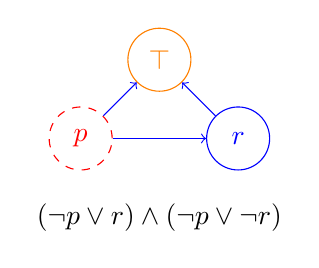
\begin{tikzpicture}
\node (p) [draw, dashed, circle, red, align=center, minimum size=0.8cm] at (0,0) {$p$};
\node (r) [draw, circle, blue, align=center, minimum size=0.8cm] at (2,0) {$r$};
\node (top) [draw, circle, orange, align=center, minimum size=0.8cm] at (1,1) {$\top$};

\draw [->, blue] (p) -- (r);
\draw [->, blue] (p) -- (top);
\draw [->, blue] (r) -- (top);

\node (formula1) [align=left] at (1,-1) {$(\lnot p \lor r) \land (\lnot p\lor \lnot r)$};

\end{tikzpicture}
\captionof{figure}{Example implication graph}
\end{center}